\documentclass[a4paper,article,14pt]{extarticle}

\usepackage{spbudiploma}
\usepackage[pdftex]{graphicx}
\usepackage{longtable}
\usepackage{makecell}
\usepackage{array}
\usepackage{float}
\usepackage{amsmath}
\usepackage{amssymb}
\usepackage{textcomp}

\graphicspath{{../images/}}
\emergencystretch=3em

\begin{document}

\newgeometry{left=30mm, top=20mm, right=15mm, bottom=20mm, nohead, nofoot}
\begin{titlepage}
\begin{center}

\textbf{Санкт-Петербургский государственный университет}

\vspace{45mm}

\textbf{\large Отчет по проекту} \\[4mm]
\textbf{\textit{\large Распределенные технологии для хранения и обработки геоданных}}

\vspace{30mm}

Выполнил: Корельский Дмитрий Сергеевич

\vfill

Санкт-Петербург\\
\the\year{} г.

\end{center}
\end{titlepage}
\restoregeometry
\addtocounter{page}{1}


\tableofcontents
\pagebreak

\specialsection{Введение}

В данном проекте рассматривается территория Ростова-на-Дону. Исходные данные
берутся из OpenStreetMap, загружаются в PostgreSQL/PostGIS при помощи
\texttt{osm2pgsql}, после чего обрабатываются набором SQL-скриптов. Финальная
визуализация подготовлена в QGIS и сохранена в проекте \path{schools_project.qgz}.

Цель работы состоит в построении контура пространственного
анализа, позволяющего:
\MList{
    \ITEM выделить объекты школ в пределах города;
    \ITEM построить зоны пешеходной доступности фиксированного радиуса;
    \ITEM найти жилые дома, попадающие в эти зоны;
    \ITEM определить ближайшие остановки общественного транспорта для школ;
    \ITEM выделить крупнейшие школьные территории;
    \ITEM найти объекты повседневного сервиса рядом со школами.
}

В рамках проекта требуется реализовать аналитический пайплайн, который
обрабатывает стандартные таблицы \texttt{osm2pgsql} и формирует производные
пространственные таблицы в отдельной схеме базы данных. В качестве входа
используются таблицы \texttt{planet\_osm\_point}, \texttt{planet\_osm\_line},
\texttt{planet\_osm\_polygon} и \texttt{planet\_osm\_roads}. В качестве выхода
необходимо получить тематические слои, пригодные для непосредственного
подключения в QGIS.

Решение включает следующие этапы:
\NList{
    \ITEM подготовка рабочей схемы \texttt{coursework};
    \ITEM поиск и фиксация административной границы Ростова-на-Дону;
    \ITEM вырезка городских данных из исходного набора OSM;
    \ITEM построение тематических выборок и производных геометрий;
    \ITEM визуализация полученных результатов в QGIS.
}

\section{Исходные данные и инструменты}

\subsection{Источник данных}

Проект опирается на данные OpenStreetMap, предварительно импортированные в
PostgreSQL при помощи \texttt{osm2pgsql}. Базовые таблицы содержат точечные,
линейные и полигональные объекты, а также упрощенный дорожный граф. Для
пространственных расчетов используется расширение PostGIS.

\subsection{Программный стек}

Для реализации проекта используется следующий набор инструментов:
\MList{
    \ITEM \texttt{PostgreSQL} как базовая СУБД;
    \ITEM \texttt{PostGIS} для хранения и обработки геометрий;
    \ITEM \texttt{osm2pgsql} для загрузки данных OSM;
    \ITEM \texttt{QGIS} для визуализации и подготовки итоговой карты;
    \ITEM \texttt{Docker Compose} для локального разворачивания окружения.
}

В файле \path{docker-compose.yaml} описан сервис \texttt{postgis} на базе
образа \texttt{postgis/postgis:18-master}. Конфигурация пробрасывает порт
\texttt{5432}, подключает каталог со скриптами \texttt{sql} и позволяет
выполнять все этапы анализа в локальном контейнере.

\section{Архитектура решения}

\subsection{Организация SQL-пайплайна}

Все вычисления разбиты на последовательность скриптов. В таблице~\ref{tab:pipeline} приведено назначение каждого
скрипта.

\begin{center}
\begin{longtable}{|>{\raggedright\arraybackslash}p{1.7cm}|>{\raggedright\arraybackslash}p{4.8cm}|>{\raggedright\arraybackslash}p{7.1cm}|}
\caption{Структура SQL-пайплайна}
\label{tab:pipeline}\\
\hline
\textbf{Шаг} & \textbf{Файл} & \textbf{Назначение} \\
\hline
\endfirsthead
\hline
\textbf{Шаг} & \textbf{Файл} & \textbf{Назначение} \\
\hline
\endhead
00 & \path{00_create_coursework_schema.sql} & Создание схемы \texttt{coursework} и проверка наличия расширения PostGIS. \\
\hline
01 & \path{01_check_public_osm_tables.sql} & Проверка состава импортированных таблиц \texttt{osm2pgsql} и их геометрических колонок. \\
\hline
02 & \path{02_find_rostov_boundary_candidates.sql} & Поиск кандидатов на административную границу Ростова-на-Дону в исходном слое OSM. \\
\hline
03 & \path{03_create_rostov_boundary.sql} & Формирование таблицы \texttt{coursework.rostov\_boundary} с выбранной городской границей. \\
\hline
04 & \path{04_create_rostov_osm_subsets.sql} & Вырезка городских объектов в локальные таблицы \texttt{coursework.rostov\_*}. \\
\hline
05 & \path{05_preview_rostov_osm_rows.sql} & Быстрый просмотр примеров строк из локальных таблиц после вырезки. \\
\hline
06 & \path{06_find_schools.sql} & Формирование единого точечного слоя школ из точечных и полигональных объектов. \\
\hline
07 & \path{07_school_buffers.sql} & Построение буферных зон радиусом 500 м вокруг школ. \\
\hline
08 & \path{08_buildings_within_school_buffers.sql} & Поиск жилых домов, попадающих в буферы, и привязка каждого дома к ближайшей школе. \\
\hline
09 & \path{09_nearest_stop_to_schools.sql} & Поиск ближайшей остановки к каждой школе и построение соединяющей линии. \\
\hline
10 & \path{10_top_school_areas.sql} & Расчет площади школьных территорий и отбор 10 крупнейших объектов. \\
\hline
11 & \path{11_cafes_and_pharmacies_near_schools.sql} & Поиск кафе и аптек в радиусе 500 м от школ с привязкой к ближайшей школе. \\
\hline
\end{longtable}
\end{center}

\subsection{Подход к пространственным вычислениям}

Во всех ключевых скриптах используются стандартные возможности PostGIS:
\MList{
    \ITEM \texttt{ST\_Intersects} для вырезки объектов по городской границе;
    \ITEM \texttt{ST\_PointOnSurface} для перехода от полигональных объектов к
    репрезентативным точкам;
    \ITEM \texttt{ST\_Buffer} для построения зон доступности;
    \ITEM \texttt{ST\_Distance} и \texttt{ST\_DWithin} для измерения расстояний;
    \ITEM оператор \texttt{<->} и \texttt{LATERAL JOIN} для поиска ближайшей
    остановки;
    \ITEM \texttt{ST\_Area} для расчета площади школьных территорий.
}

Геометрии хранятся в проекции EPSG:3857, однако расстояния и площади в
критических вычислениях приводятся к типу \texttt{geography} через преобразование
в EPSG:4326. Это позволяет получать значения в метрах и квадратных метрах, что
важно для корректной интерпретации результатов.

\section{Реализация анализа}

\subsection{Выделение городской территории}

Скрипты \texttt{02} и \texttt{03} отвечают за извлечение административной
границы Ростова-на-Дону из слоя \path{planet_osm_polygon}. Сначала
формируется список кандидатов по тегам \texttt{boundary = administrative},
названию и \texttt{admin\_level}. Затем выбирается один объект, приоритетно
соответствующий городскому округу Ростов-на-Дону.

После фиксации границы скрипт \texttt{04} создает локальные таблицы
\path{coursework.rostov_point}, \path{coursework.rostov_line},
\path{coursework.rostov_polygon} и \path{coursework.rostov_roads}. В них
остаются только объекты, пересекающие выбранную городскую территорию. На каждую
таблицу создается пространственный индекс \texttt{GIST}, после чего выполняется
\texttt{ANALYZE}.

\subsection{Формирование слоя школ}

Скрипт \texttt{06\_find\_schools.sql} собирает школы из двух источников:
точечных и полигональных объектов. Для полигонов используется функция
\texttt{ST\_PointOnSurface}, позволяющая перевести площадной объект в точку,
пригодную для последующих вычислений расстояний и буферов.

Итоговый слой \texttt{coursework.schools} содержит:
\MList{
    \ITEM уникальный идентификатор \texttt{gid};
    \ITEM исходный \texttt{osm\_id};
    \ITEM название школы;
    \ITEM значение поля \texttt{amenity};
    \ITEM признак источника: \texttt{point} или \texttt{polygon};
    \ITEM точечную геометрию объекта.
}

\subsection{Буферные зоны и жилая застройка}

Скрипт \texttt{07\_school\_buffers.sql} строит буферы радиусом 500 метров вокруг
каждой школы. Буферы формируются в метрической интерпретации через тип
\texttt{geography}, а затем возвращаются к геометрии EPSG:3857. Полученная
таблица \texttt{coursework.school\_buffers} является базой для последующего
анализа доступности.

Скрипт \path{08_buildings_within_school_buffers.sql} выбирает жилые дома по
списку характерных значений поля \texttt{building}, определяет их пересечение с
буферами и сопоставляет каждый дом с ближайшей школой внутри допустимого радиуса.
Для этого сначала формируются все совпадения дом-школа, затем из них остается
одна запись с минимальным расстоянием до школы.

\subsection{Остановки и сервисные объекты}

Скрипт \texttt{09\_nearest\_stop\_to\_schools.sql} определяет ближайшую остановку
общественного транспорта для каждой школы. В выборку включаются автобусные
остановки, платформы и некоторые железнодорожные объекты. Поиск ближайшего
соседа выполняется через \texttt{LEFT JOIN LATERAL} и сортировку по оператору
\texttt{<->}, после чего между школой и остановкой строится линия
\texttt{ST\_MakeLine}.

Скрипт \texttt{11\_cafes\_and\_pharmacies\_near\_schools.sql} ищет кафе и аптеки в
радиусе 500 метров от школ. Источником служат как точечные, так и полигональные
объекты. Для полигонов также используется \texttt{ST\_PointOnSurface}, а итогом
является таблица, в которой каждый сервисный объект связан с ближайшей школой в
указанном радиусе.

\subsection{Ранжирование школьных территорий}

Скрипт \texttt{10\_top\_school\_areas.sql} работает только с полигональными
школьными объектами. Для каждого объекта рассчитывается площадь в квадратных
метрах, после чего выполняется ранжирование по убыванию площади. В итоговую
таблицу \texttt{coursework.top\_school\_areas} попадают десять крупнейших
территорий.

\section{Результаты визуализации}

Итоговые слои подключены в QGIS-проект \path{schools_project.qgz}. Ниже
приведены основные карты, демонстрирующие результаты анализа.

\begin{figure}[H]
\begin{center}
\includegraphics[width=\textwidth]{demo.png}
\caption{Общий вид проекта в QGIS}
\label{fig:demo}
\end{center}
\end{figure}

На рисунке~\ref{fig:demo} показана сводная карта проекта. На ней одновременно
присутствуют школы, буферные зоны, жилые дома, ближайшие остановки и сервисные
объекты. Такой слой удобен для визуальной проверки корректности пайплайна и
согласованности тематических таблиц.

\begin{figure}[H]
\begin{center}
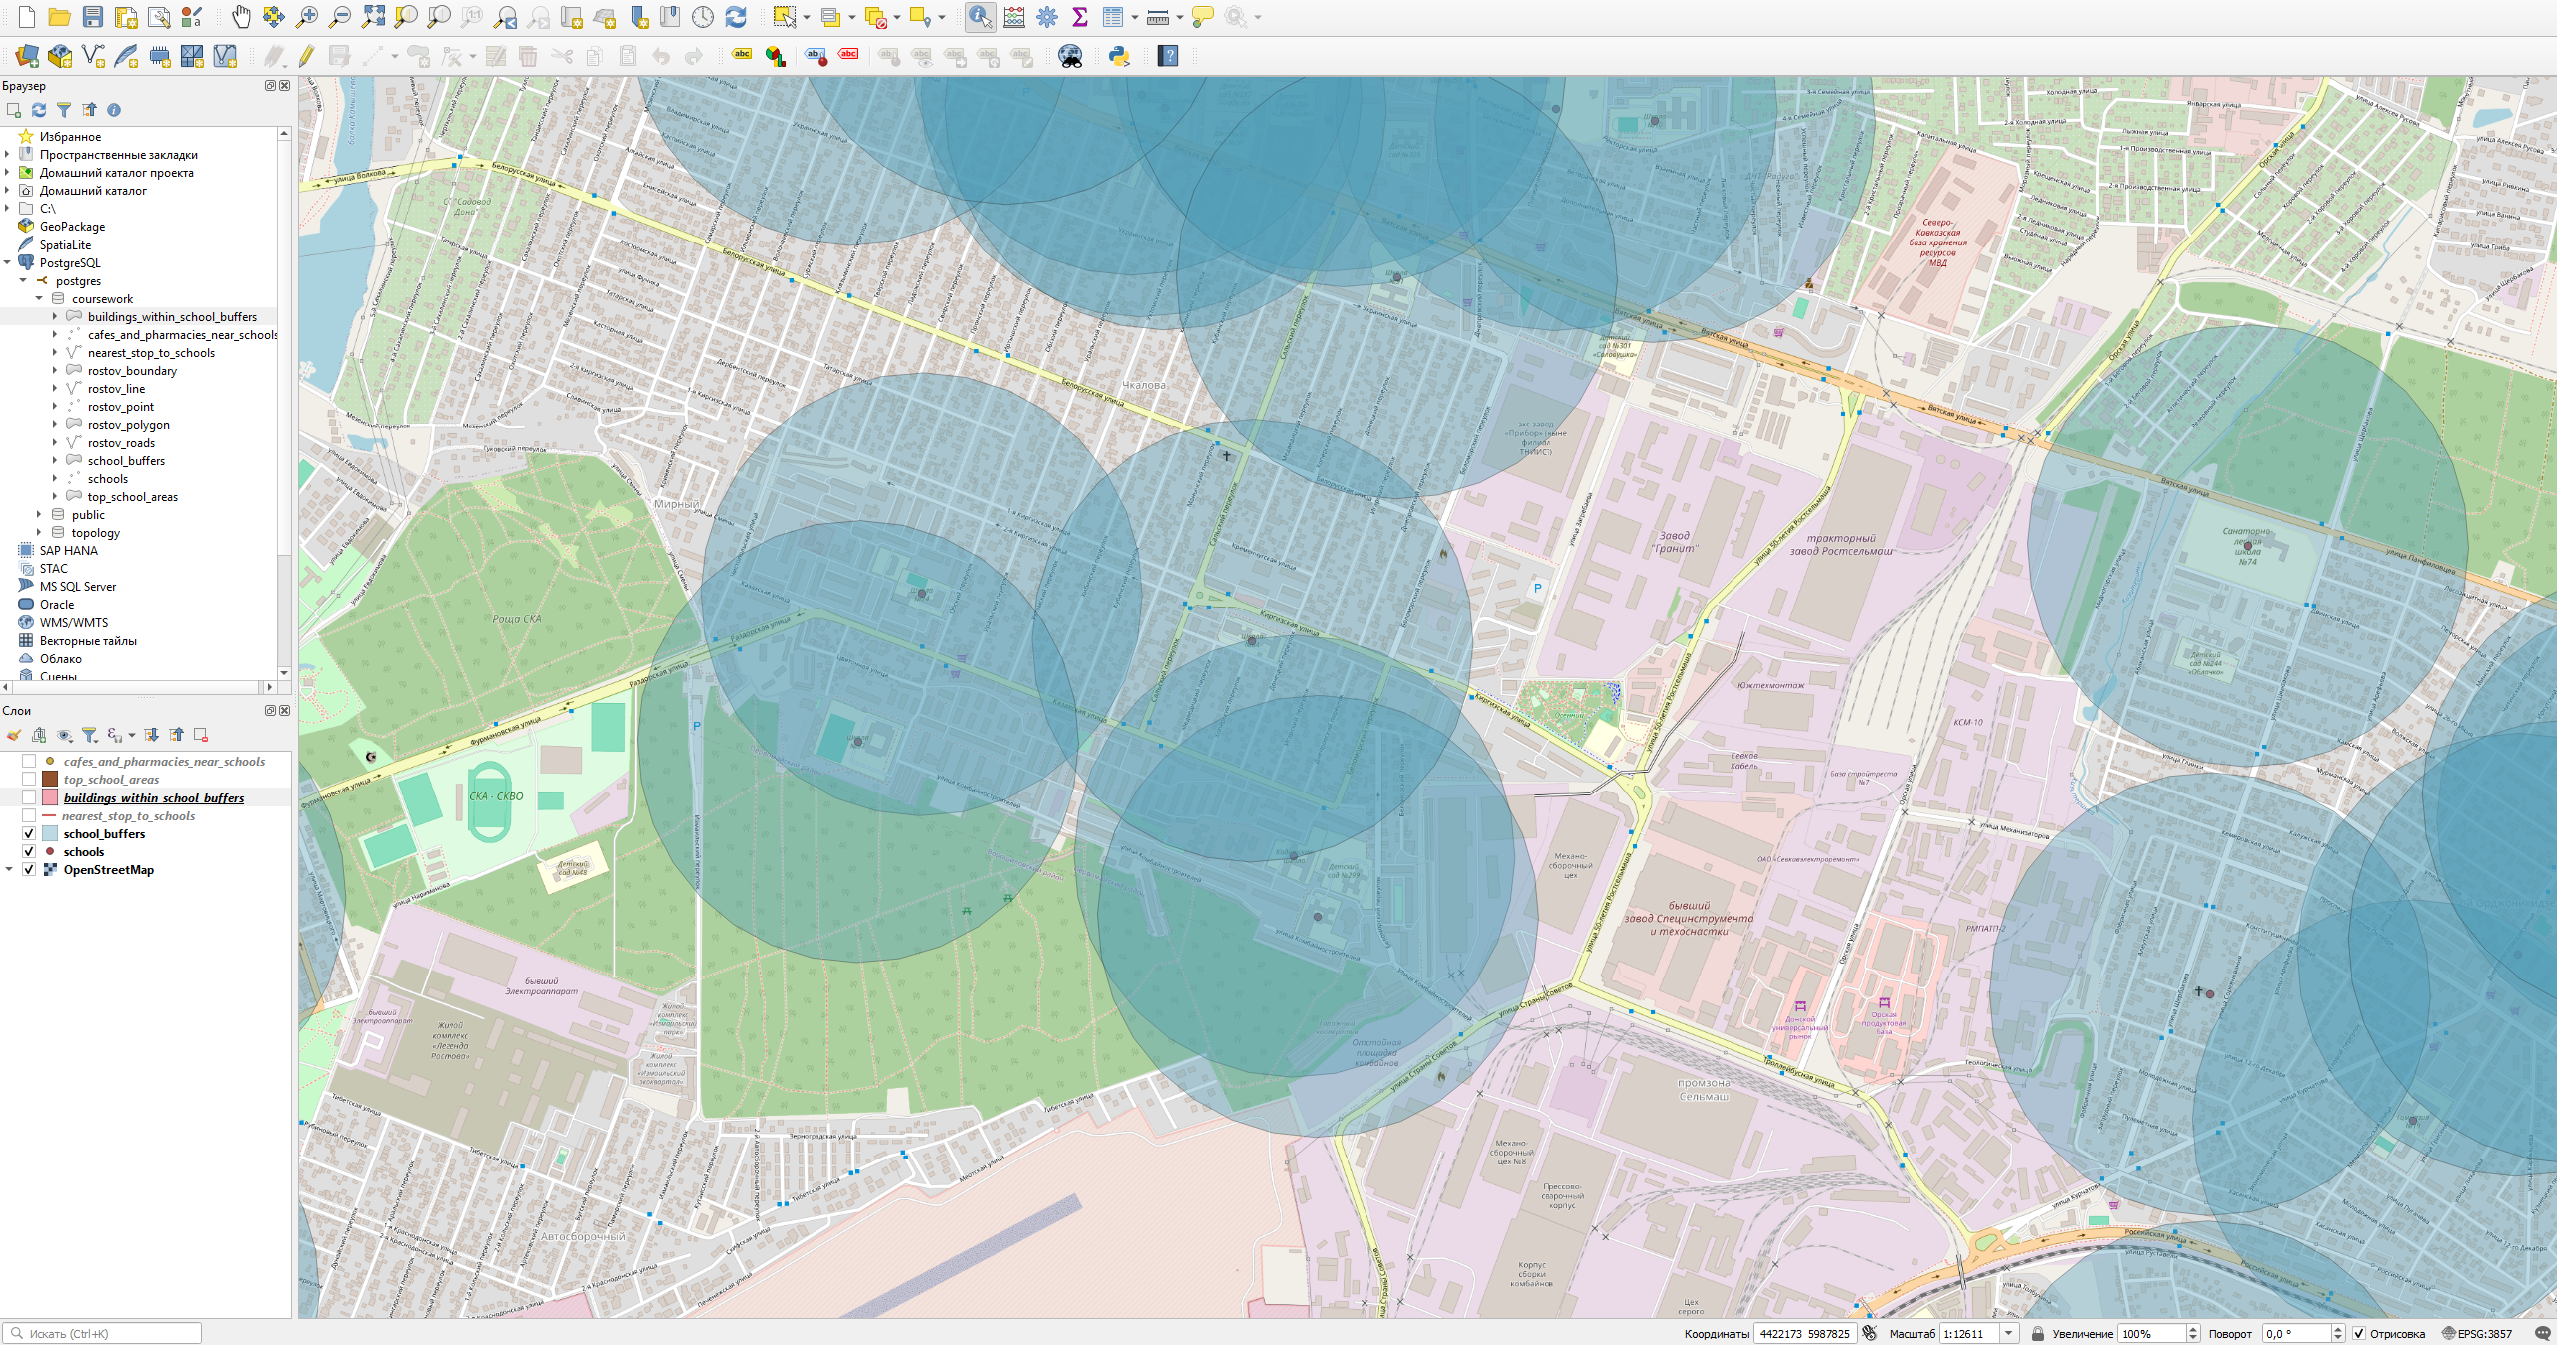
\includegraphics[width=\textwidth]{schools_and_buffers.png}
\caption{Школы и буферные зоны радиусом 500 метров}
\label{fig:buffers}
\end{center}
\end{figure}

Рисунок~\ref{fig:buffers} показывает базовый результат построения зон доступности
вокруг школ. Эти полигоны выступают опорным слоем для дальнейшего анализа жилой
застройки.

\begin{figure}[H]
\begin{center}
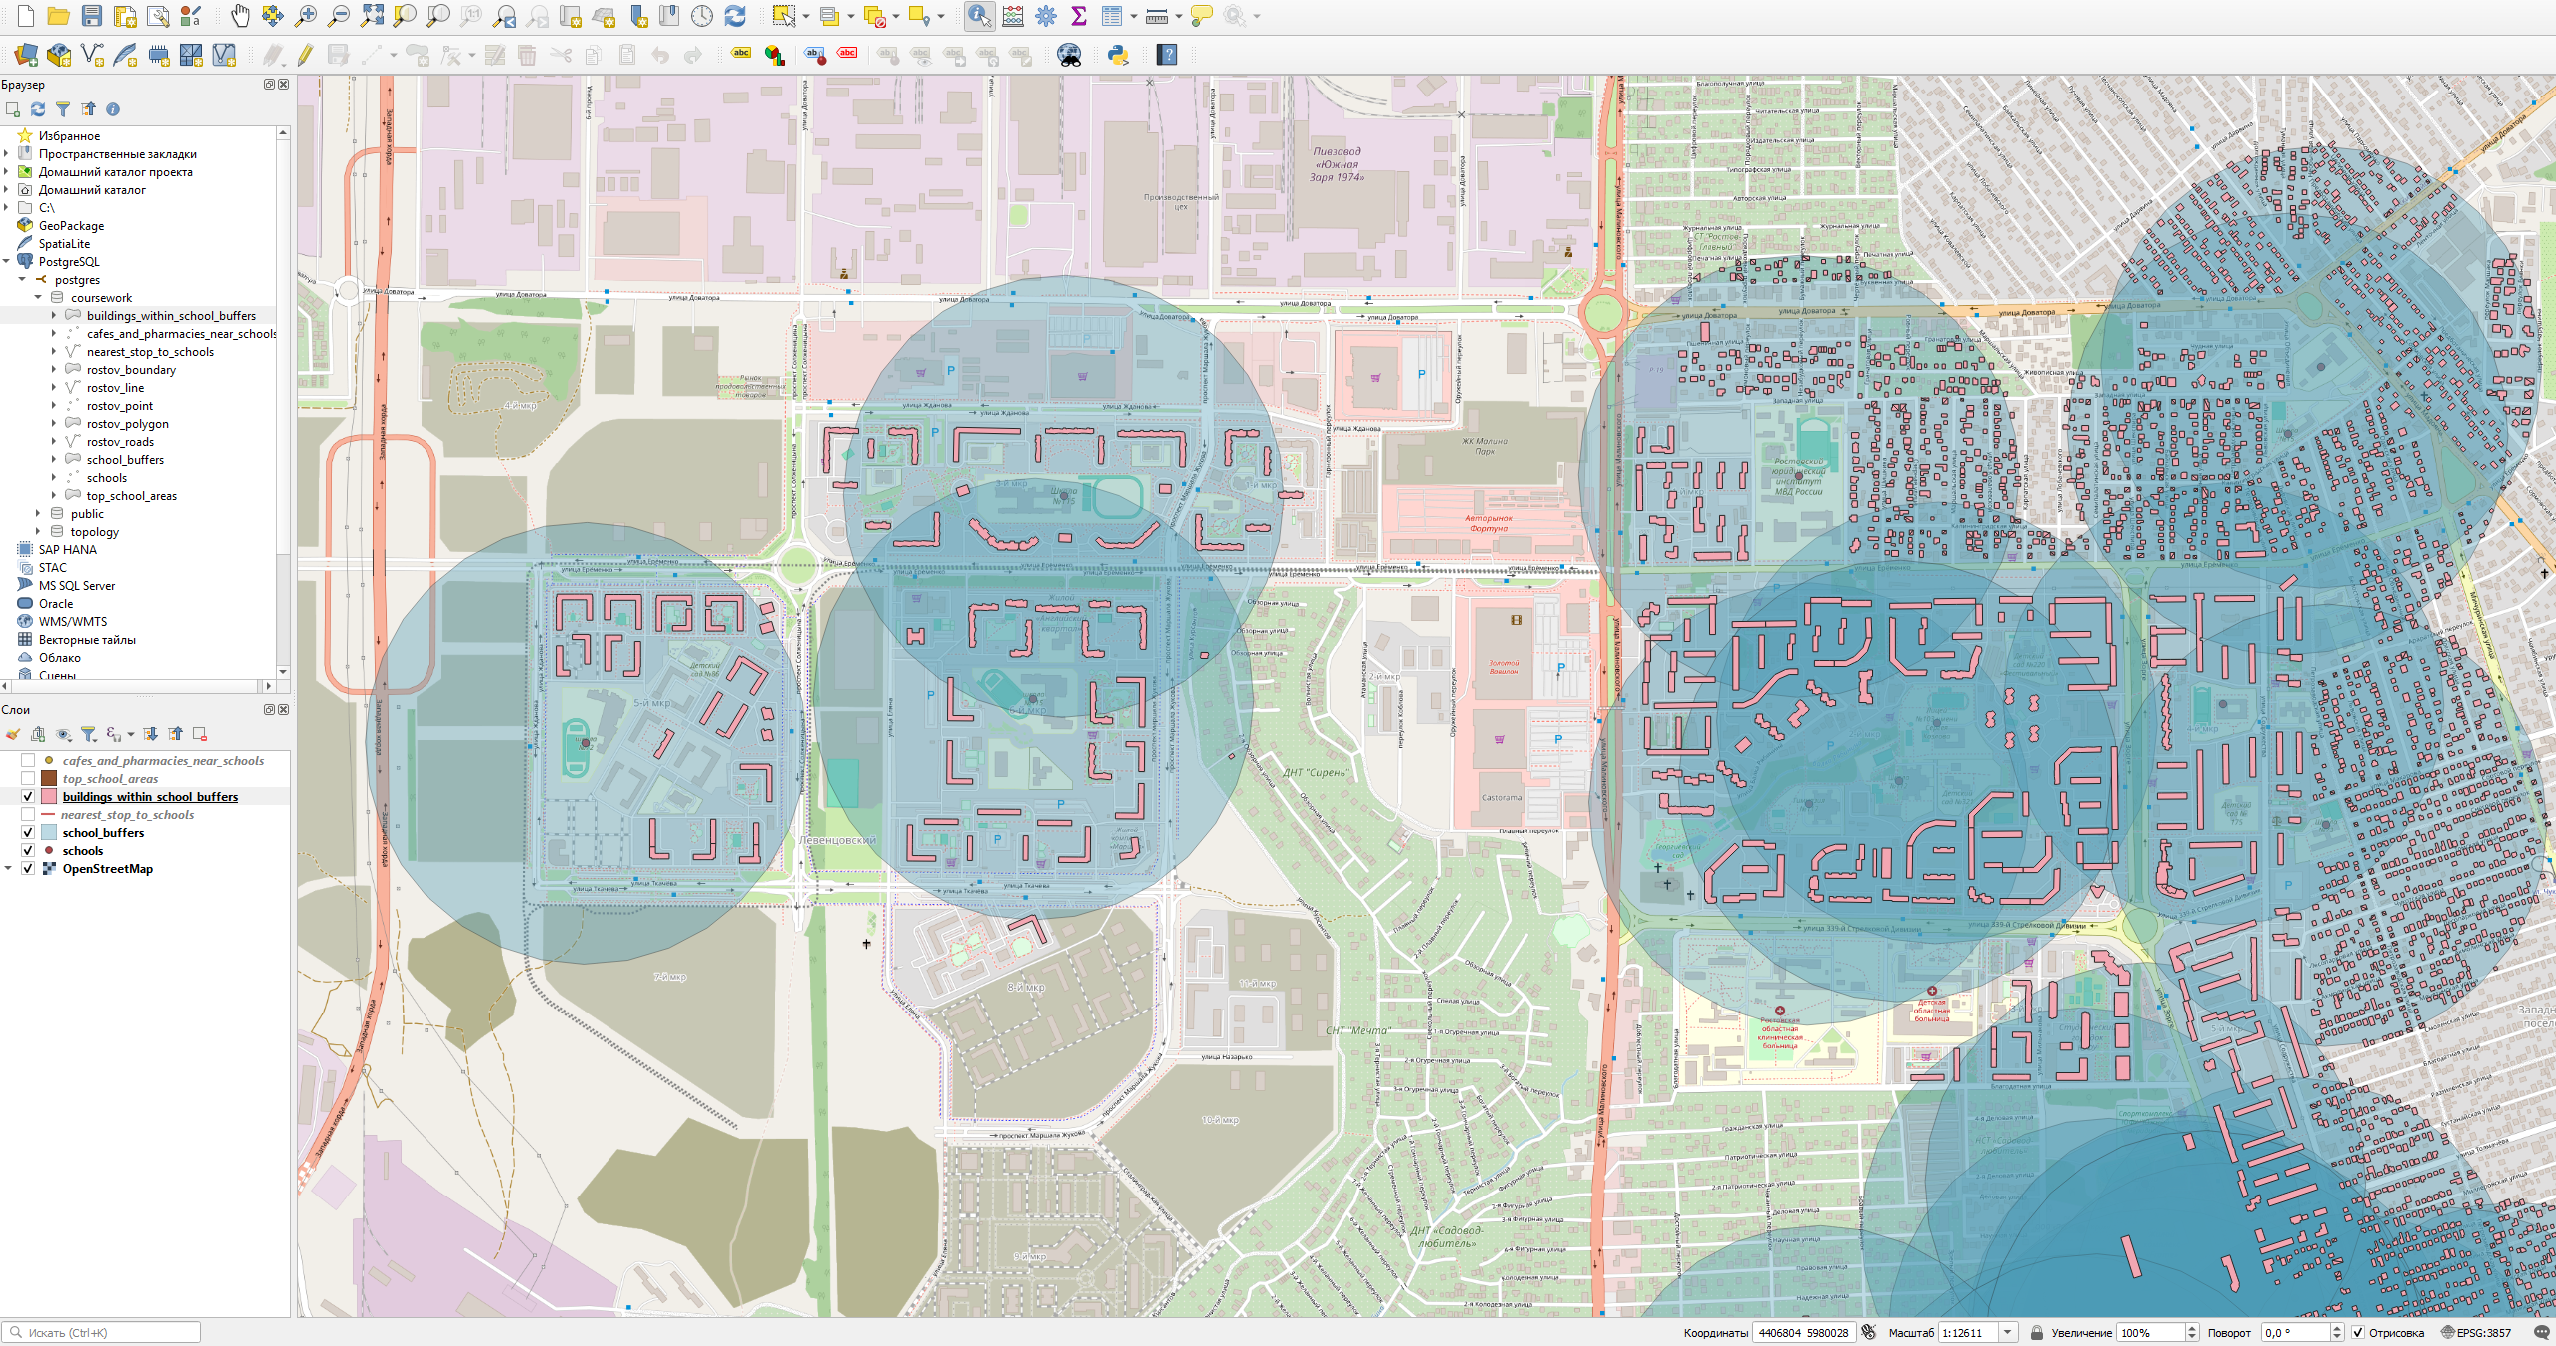
\includegraphics[width=\textwidth]{apartments_near_schools.png}
\caption{Жилые дома, расположенные рядом со школами}
\label{fig:apartments}
\end{center}
\end{figure}

На рисунке~\ref{fig:apartments} отображаются жилые дома, попавшие в буферы
доступности. В аналитической таблице для каждого здания дополнительно хранится
расстояние до ближайшей школы.

\begin{figure}[H]
\begin{center}
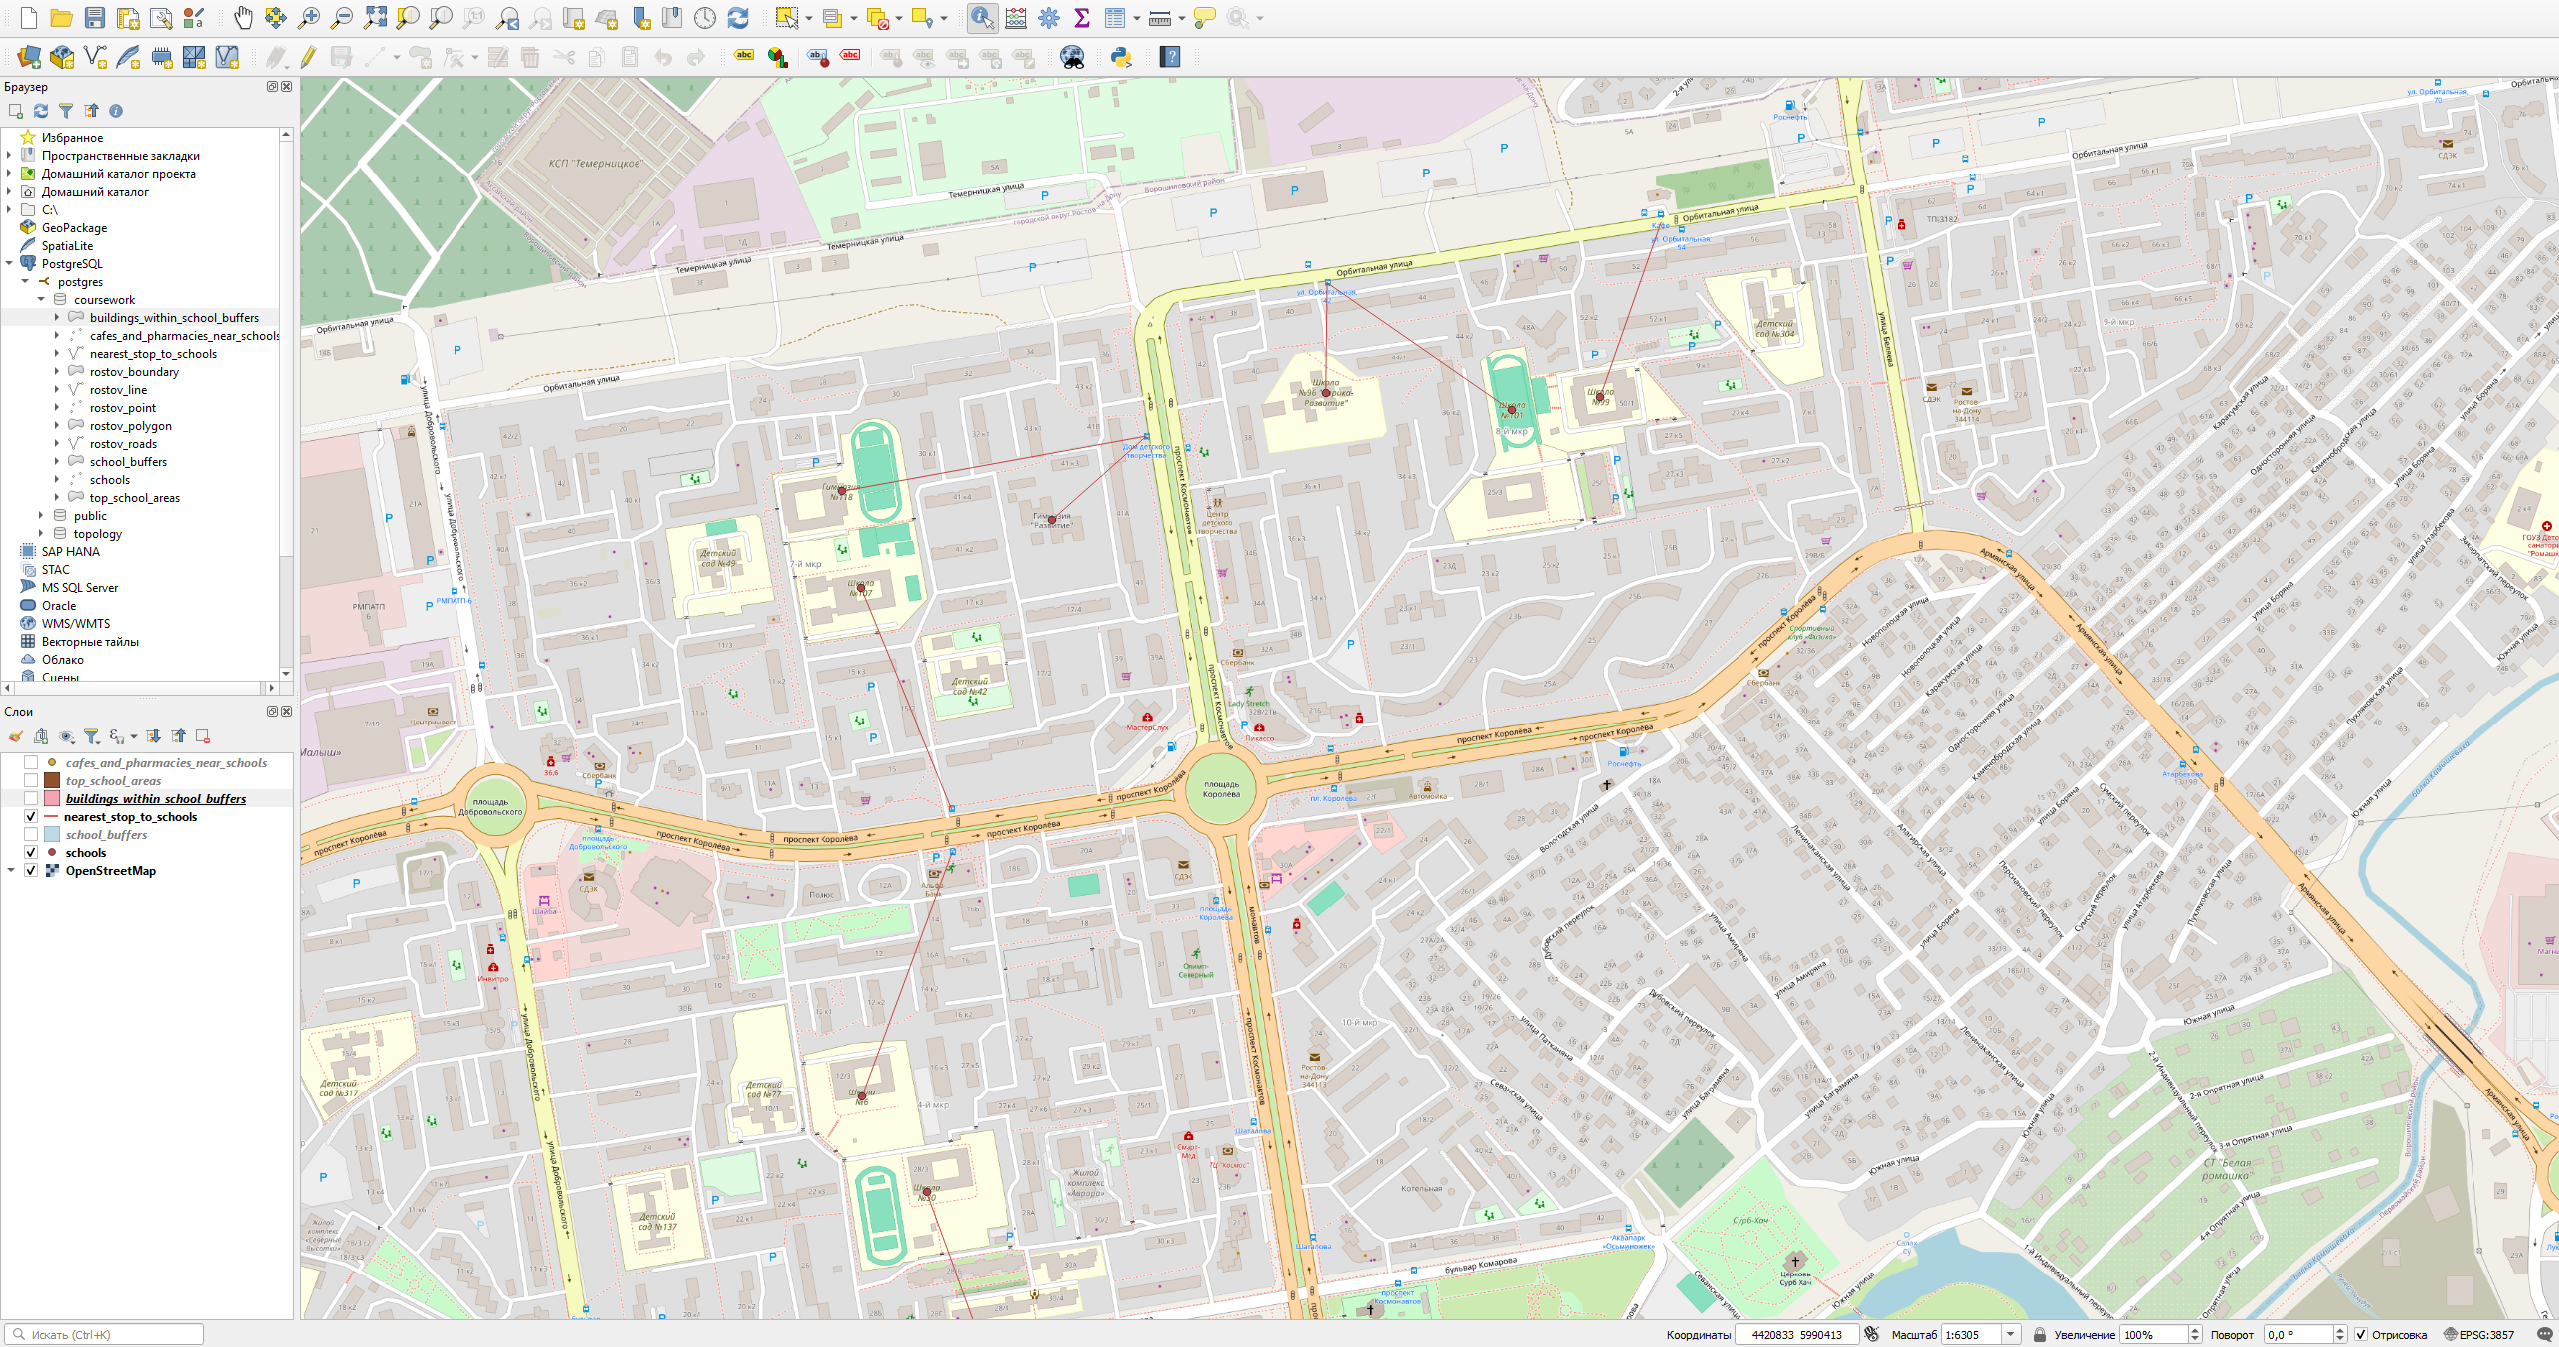
\includegraphics[width=\textwidth]{nearest_bus_stops.png}
\caption{Ближайшие остановки общественного транспорта для школ}
\label{fig:stops}
\end{center}
\end{figure}

Рисунок~\ref{fig:stops} демонстрирует результат поиска ближайших остановок.
Соединяющие линии позволяют быстро выявлять школы с более сложной транспортной
доступностью.

\begin{figure}[H]
\begin{center}
\includegraphics[width=\textwidth]{top_schools_areas.png}
\caption{Крупнейшие школьные территории}
\label{fig:areas}
\end{center}
\end{figure}

Рисунок~\ref{fig:areas} иллюстрирует результат ранжирования школьных территорий
по площади. Этот слой может использоваться как база для дальнейшего анализа
емкости школьной инфраструктуры.

\begin{figure}[H]
\begin{center}
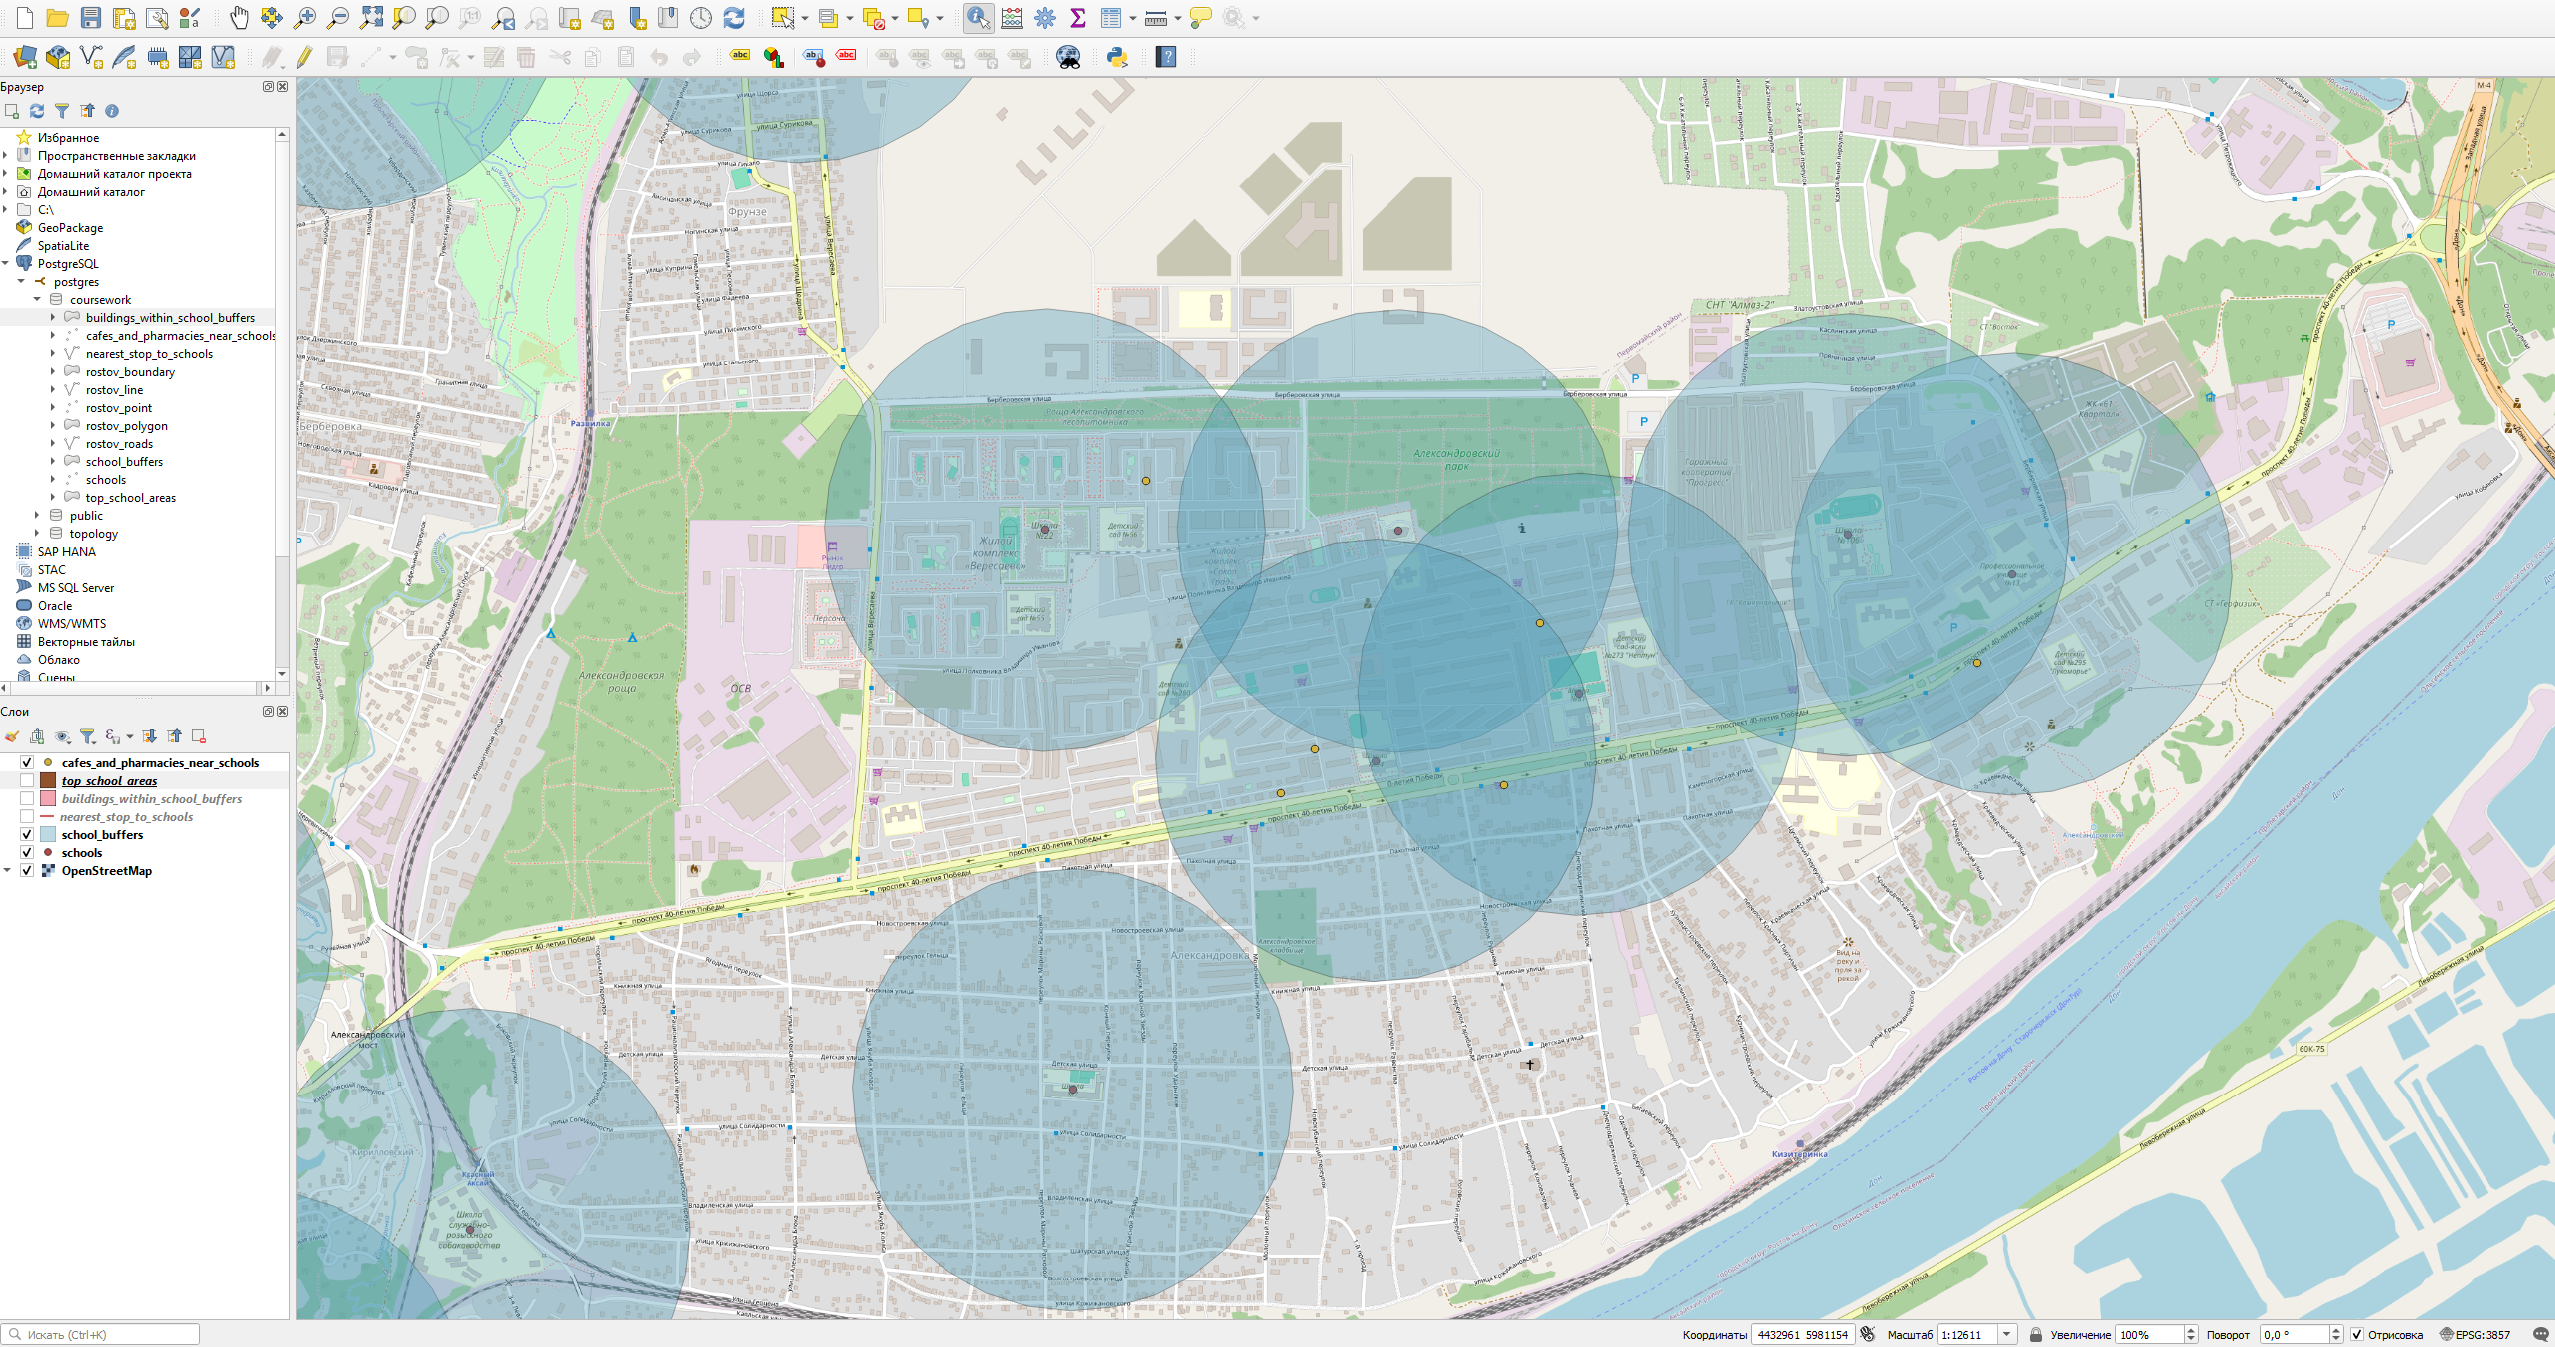
\includegraphics[width=\textwidth]{cafes_and_pharmaces_near_schools.png}
\caption{Кафе и аптеки вблизи школ}
\label{fig:services}
\end{center}
\end{figure}

На рисунке~\ref{fig:services} показаны объекты повседневного сервиса,
расположенные рядом со школами. Эта карта полезна для качественной оценки
окружения школьной инфраструктуры.

\specialsection{Выводы}

В ходе работы был подготовлен воспроизводимый проект пространственного анализа
доступности школ в Ростове-на-Дону на базе \texttt{PostGIS + QGIS}. Реализованный
SQL-пайплайн формирует отдельную рабочую схему, вырезает городские объекты из
общего набора OSM и строит тематические аналитические таблицы.

Ключевыми результатами являются:
\MList{
    \ITEM слой школ, приведенный к единому точечному представлению;
    \ITEM буферные зоны радиусом 500 метров;
    \ITEM слой жилых домов, находящихся рядом со школами;
    \ITEM линии до ближайших остановок общественного транспорта;
    \ITEM выборка крупнейших школьных территорий;
    \ITEM слой кафе и аптек в радиусе 500 метров от школ.
}

\end{document}
